\documentclass[a4paper, fleqn]{article}

\usepackage{amsmath}
\usepackage{enumitem}
\usepackage{graphicx}

\begin{document}

\title{Lab Exercise I \\ Making Maps I: Introduction to Spatial Analysis, Data Visualization and Map Design}
\author{Basil R. Yap}
\date{2018 January 25}
\maketitle

\begin{enumerate}

\item \textbf{Distance between Singapore and Taipei: }3,297.421 km
\item \textbf{Estimated population of Afghanistan: }34124811
\item \textbf{Country with the 5th highest GDP: }Germany

\end{enumerate}

\pagebreak

\section{Map Assignment}
A copy of this map is contained within the folder alongside this document.
\begin{figure}[h!]
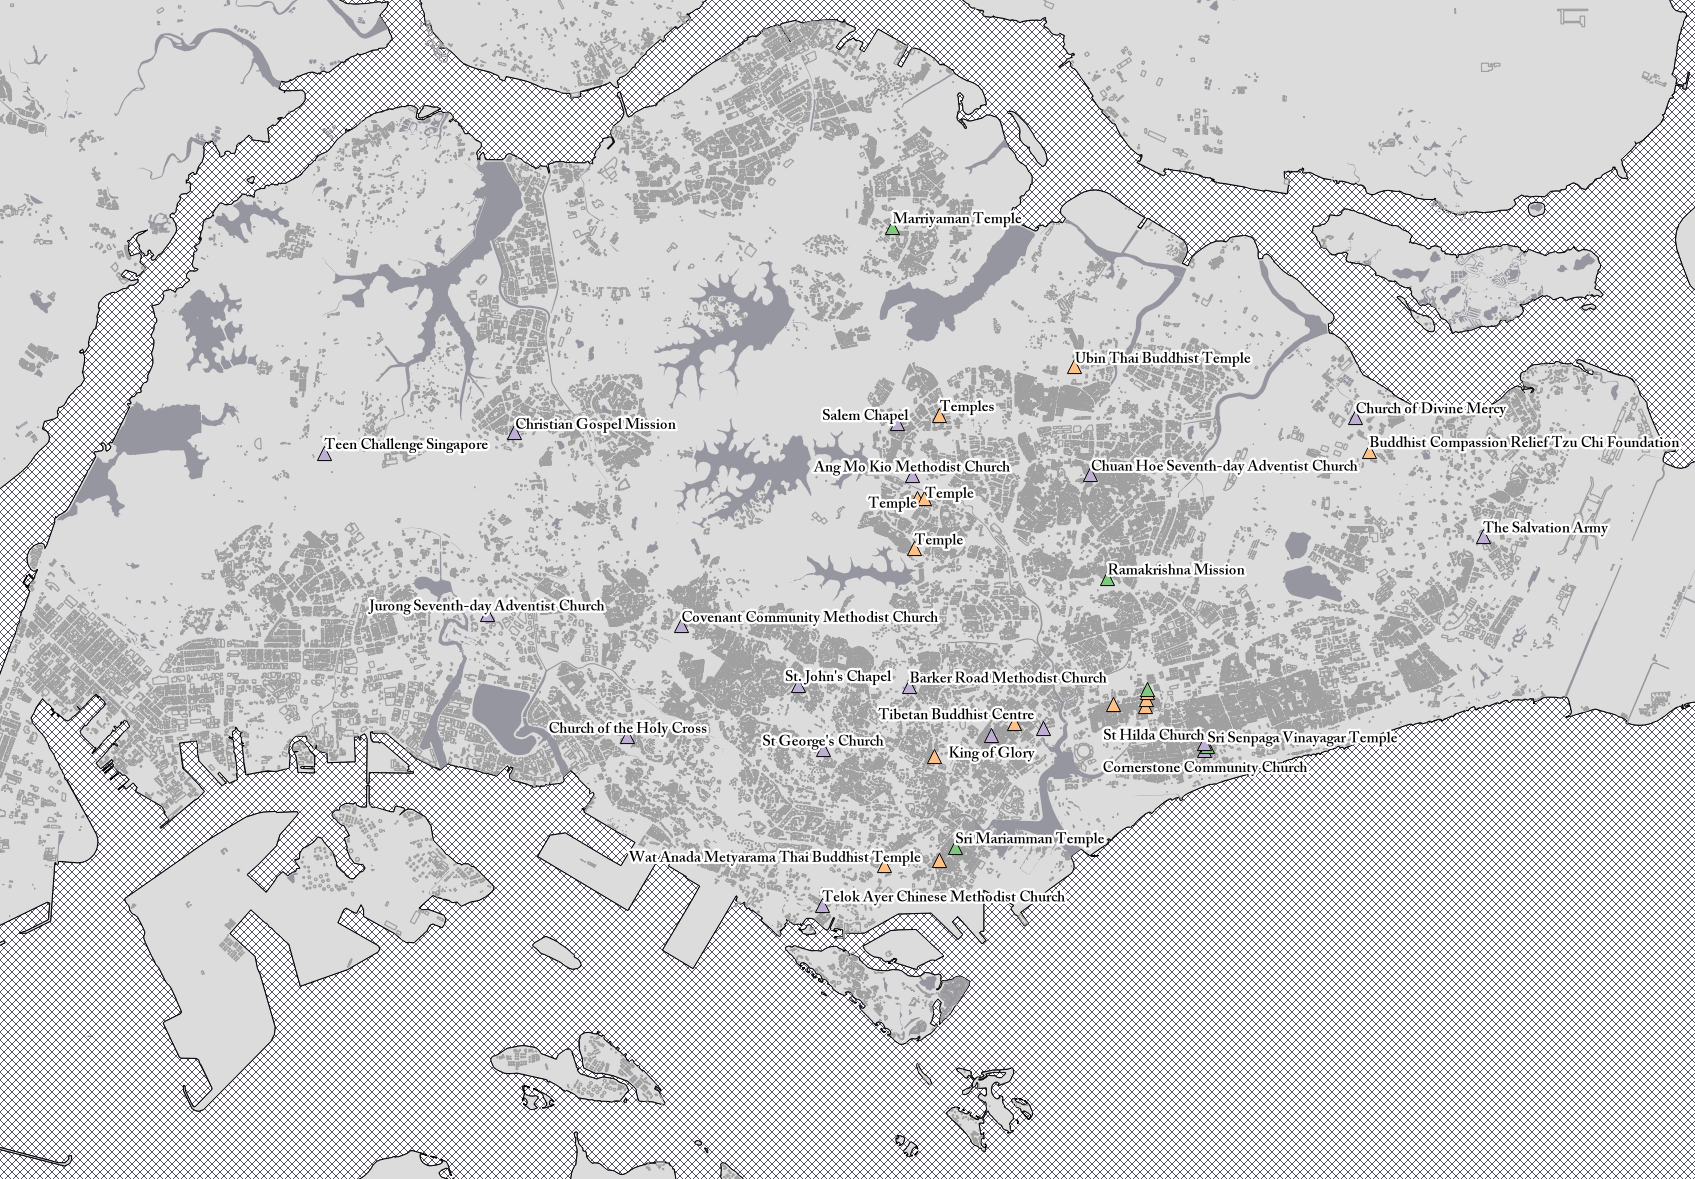
\includegraphics[width=\linewidth]{assets/201801311741.png}
\caption{Distribution of Places of Worship in Singapore}
\label{fig:map1}
\end{figure}

\textbf{Goal of the Map: }Show in a concise manner, the distribution of religious establishments across Singapore and possibly deducing the concentration of people practicing each religion at various parts of the island.\\

\textbf{Decisions made in the making of this map:}
\begin{enumerate}
\item \textbf{Changing the external waters to a plain hash:}\\
Shift the attention of the viewer towards the Singapore landmass and the points of interest contained within it.
\item \textbf{Removal of irrelevant content(i.e. roads, foliage, etc.):}\\
Elements that were not relevant to the analysis were removed in order to improve readability of the map. It is worth noting, buildings were left in the map to allow viewers to infer the location of residential sectors.
\item \textbf{Visualizing locations of Religious Establishments: }\\
Qualitative colors were selected using colorbrewer.com and the rest of the map was left in gray-scale. This allowed the three religious entities contained in the data to be easily while drawing in the viewer's attention by standing out on the map.
\end{enumerate}

\end{document}